\documentclass[conference]{IEEEtran}
\usepackage{graphicx}
\usepackage{booktabs}
\usepackage{array}
\usepackage{url}
\usepackage[hidelinks]{hyperref}
\usepackage{listings}
\lstset{basicstyle=\ttfamily\footnotesize,columns=fullflexible,breaklines=true,frame=single,xleftmargin=2pt,xrightmargin=2pt}
\graphicspath{{../}{../../evidence/phase1/A-network/}{../../evidence/phase1/B-dns/}{../../evidence/phase1/D-loadbalancer/}{../../evidence/phase1/E-https/}{../../evidence/phase1/F-caching/}{../../evidence/phase1/G-wireshark/}{../../evidence/phase1/failures/}}
\newcommand{\cmd}[1]{\texttt{#1}}
\makeatletter\g@addto@macro{\UrlBreaks}{\do\-\do\_}\makeatother
\newcommand{\src}[1]{\\\footnotesize\textit{Source:} \nolinkurl{evidence/phase1/#1}}
\newcommand{\srcp}[1]{\\\footnotesize\textit{Source:} \nolinkurl{#1}}

\begin{document}

\title{Building and Observing a Private Service Network:\\ DNS, Reverse-Proxy Load Balancing, TLS and Caching on Two Laptops}

\author{\IEEEauthorblockN{Yatin Singh}
\IEEEauthorblockA{\textit{B.Tech CS \& AI}\\
\textit{Newton School of Technology}\\
\textit{Rishihood University}}
\and
\IEEEauthorblockN{Dadi Dinesh}
\IEEEauthorblockA{\textit{B.Tech CS \& AI}\\
\textit{Newton School of Technology}\\
\textit{Rishihood University}}}

\maketitle

\begin{abstract}
This report describes Phase~1 of a Computer Networks course project: a private service network built from scratch on two macOS laptops sharing one Wi-Fi hotspot, with no cloud services. A client resolves the private name \cmd{app.team1.test} through our own dnsmasq resolver, opens an HTTPS connection to an nginx reverse proxy that terminates TLS with a certificate signed by a local certificate authority, and is load-balanced across two Express backends. One endpoint demonstrates HTTP caching with \cmd{Cache-Control} and ETag revalidation. Every step of a single request---DNS over UDP port 53, the TCP three-way handshake, the TLS handshake and encrypted application data---was captured with Wireshark, and five deliberate failures were used to show which layer each fault affects. Each claim in the report references a screenshot in the project's evidence folder.
\end{abstract}

\begin{IEEEkeywords}
DNS, dnsmasq, nginx, reverse proxy, load balancing, TLS, certificate authority, HTTP caching, Wireshark, TCP
\end{IEEEkeywords}

\section{Introduction}
A browser request to a web service relies on several independent layers: the name is resolved to an address, a TCP connection is opened to a port on that address, a TLS session is negotiated over it, and only then is HTTP exchanged. Cloud platforms hide these layers behind managed services. The goal of this project is to build each of them by hand and to prove, with tools, what happens at each step.

By the end of Phase~1, a client on our network had to type \cmd{https://app.team1.test}, resolve it through our own DNS server, connect securely through our reverse proxy, and receive a response from one of two backends, with packet-level evidence of the whole path. The brief divides this into seven tasks (A--G) and five failure demonstrations; Sections~\ref{sec:arch}--\ref{sec:fail} follow that order. Section~\ref{sec:lessons} discusses what we learned, including a host-level firewall problem that shaped our topology.

\section{Architecture and LAN (Task A)}\label{sec:arch}
\subsection{Topology}
The team has two members and two laptops; the brief allows small teams to combine roles. Table~\ref{tab:roles} and Fig.~\ref{fig:topo} show the result. Mac~2 hosts the DNS resolver, the nginx edge and both backends; Mac~1 is the client. Each role corresponds to a cloud service: dnsmasq plays the part of a managed DNS service such as Route~53, nginx that of a cloud load balancer such as AWS ALB, and the backends that of application server instances.

\begin{table}[htbp]
\caption{Machine Roles, Addresses and Services}
\label{tab:roles}
\centering
\begin{tabular}{@{}l l l l@{}}
\toprule
Host & Role & Address & Service / port \\
\midrule
Mac 1 & Client & 10.166.26.230 (en0) & browser, curl, dig \\
Mac 2 & DNS & 10.166.26.178 (en0) & dnsmasq, UDP 53 \\
Mac 2 & Edge & 10.166.26.178 (en0) & nginx, TCP 443, 80 \\
Mac 2 & Backend A & 127.0.0.1 (lo0) & Express, TCP 4000 \\
Mac 2 & Backend B & 127.0.0.1 (lo0) & Express, TCP 6000 \\
\bottomrule
\end{tabular}
\end{table}

\begin{figure}[htbp]
\centerline{\includegraphics[width=\columnwidth]{topology.png}}
\caption{Topology and request flow: (1) DNS query, (2) TCP handshake, (3) TLS handshake, (4) encrypted request, (5) plain HTTP to a backend, (6) encrypted response.\srcp{docs/topology.png}}
\label{fig:topo}
\end{figure}

\subsection{LAN Verification}
Both laptops obtained addresses from the hotspot by DHCP. Fig.~\ref{fig:netinfo} shows that they share the subnet mask 255.255.255.0 and the default gateway, so they are on one LAN segment, and Fig.~\ref{fig:ping} shows reachability in both directions with no packet loss. These screenshots were taken on an earlier session of the same hotspot setup (10.198.95.0/24); the hotspot assigns a new subnet on reconnection, so later evidence uses 10.166.26.0/24.

\begin{figure}[htbp]
\centering
\includegraphics[width=\columnwidth]{A-mac2-server-network-info.png}\\[3pt]
\includegraphics[width=\columnwidth]{A-mac1-client-network-info.jpeg}
\caption{Interface, address, mask, gateway and MAC address of Mac~2 (top) and Mac~1 (bottom).\src{A-network/}}
\label{fig:netinfo}
\end{figure}

\begin{figure}[htbp]
\centering
\includegraphics[width=\columnwidth]{A-ping-mac2-to-mac1.png}\\[3pt]
\includegraphics[width=\columnwidth]{A-ping-mac1-to-mac2.jpeg}
\caption{Ping from Mac~2 to Mac~1 (top) and from Mac~1 to Mac~2 (bottom), 0\% packet loss.\src{A-network/}}
\label{fig:ping}
\end{figure}

\section{Private DNS (Task B)}
Mac~2 runs dnsmasq~\cite{dnsmasq} with the configuration in Fig.~\ref{fig:dnsconf}. The \cmd{address=} lines map \cmd{app.team1.test} and \cmd{api.team1.test} to Mac~2; \cmd{local=/team1.test/} keeps the zone from being forwarded; all other names are forwarded to 8.8.8.8 and 1.1.1.1 so that ordinary browsing works; \cmd{listen-address} binds both loopback and the LAN address; and \cmd{local-ttl=30} sets a 30-second TTL~\cite{rfc1034}. We chose the \cmd{.test} top-level domain because it is reserved~\cite{rfc6761}: a public resolver answers NXDOMAIN for it, so it cannot clash with a real name.

\begin{figure}[htbp]
\centerline{\includegraphics[width=\columnwidth]{B-dnsmasq-config.png}}
\caption{dnsmasq configuration on Mac~2.\src{B-dns/B-dnsmasq-config.png}}
\label{fig:dnsconf}
\end{figure}

Fig.~\ref{fig:dig} shows the resolver's answer: status \cmd{NOERROR}, the \cmd{aa} (authoritative) flag, and \cmd{app.team1.test 30 IN A 10.166.26.178}. This query was made on Mac~2 itself; the same lookup from the client, Mac~1, appears at packet level in Fig.~\ref{fig:wsdns} (query from 10.166.26.230 to 10.166.26.178 on UDP port 53) and in the first lines of Fig.~\ref{fig:curl}, where curl on Mac~1 resolves the name to 10.166.26.178. Resolution only yields an address; the TCP and TLS connection that follows is a separate step.

\begin{figure}[htbp]
\centerline{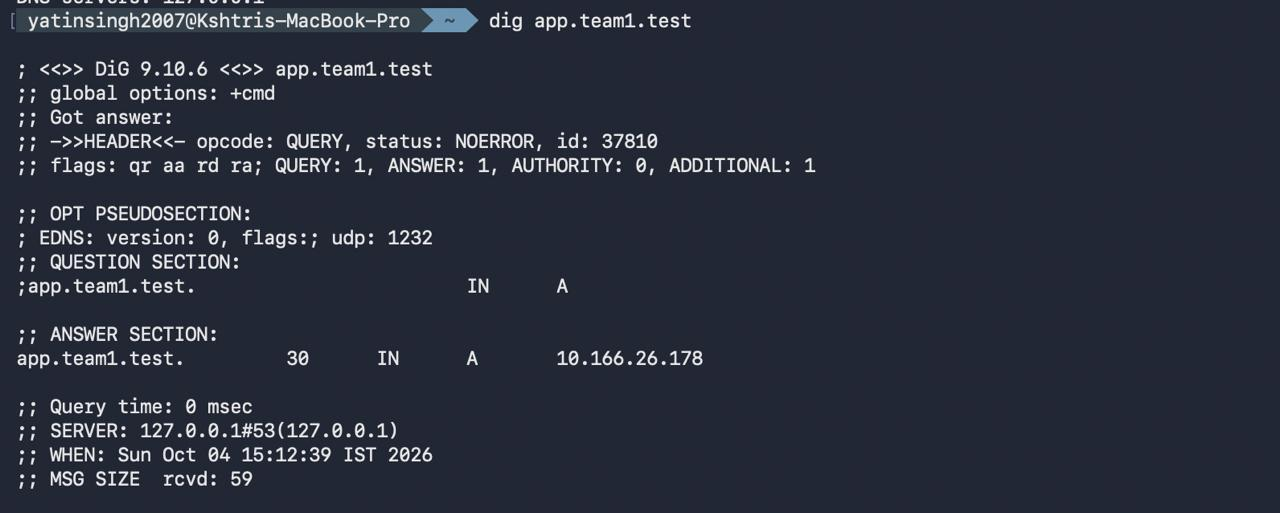
\includegraphics[width=\columnwidth]{B-dig.png}}
\caption{\cmd{dig app.team1.test}: authoritative answer with TTL 30.\src{B-dns/B-dig.png}}
\label{fig:dig}
\end{figure}

\section{Backends, Reverse Proxy and Load Balancing (Tasks C and D)}
Each backend is a small Express~\cite{express} application. \cmd{GET /} returns \cmd{hello from backend A} or \cmd{hello from backend B}, identifying the server that answered, and \cmd{GET /api/data} returns a fixed JSON document used for the caching test. Backend~A listens on port 4000 and Backend~B on port 6000.

nginx on Mac~2 is the single entry point. Its upstream block lists both backends; round-robin is nginx's default strategy~\cite{nginxup}:
\begin{lstlisting}
upstream team1_backends {
  server 127.0.0.1:4000 max_fails=1 fail_timeout=10s;
  server 127.0.0.1:6000 max_fails=1 fail_timeout=10s;
}
location / {
  proxy_pass http://team1_backends;
  proxy_next_upstream error timeout http_502 http_503;
}
\end{lstlisting}
Fig.~\ref{fig:rr} shows six requests from Mac~1 alternating between the backends. The client never needs the backend addresses: DNS gives it only the edge's address, and nginx alone knows the upstream pool, so backends can be added or replaced without changing clients. Browsers also request \cmd{/favicon.ico} on every page load, which made the page itself always land on the same backend; answering that path directly in nginx (\cmd{return 204}) made the browser view alternate as well.

\begin{figure}[htbp]
\centerline{\includegraphics[width=\columnwidth]{D-roundrobin.png}}
\caption{Six consecutive requests from Mac~1 alternate between Backend A and Backend B.\src{D-loadbalancer/D-roundrobin.png}}
\label{fig:rr}
\end{figure}

\section{HTTPS and TLS (Task E)}
Using OpenSSL we created a local certificate authority (``Team1 Local CA'', \cmd{CA:TRUE}) and a server key, and signed a certificate for \cmd{app.team1.test} with both project names in the Subject Alternative Name extension, which browsers use for name matching instead of the common name. nginx serves it on port 443 with TLS~1.2 and 1.3 enabled and redirects port 80 to HTTPS with a 301. The CA certificate was added to the client's system trust store; only public certificates are committed to the repository, and private keys are excluded by \cmd{.gitignore}.

Fig.~\ref{fig:curl} is \cmd{curl -v} from Mac~1, without \cmd{-k}. It shows the TCP connection to port 443, the TLS~1.3 handshake (ClientHello, ServerHello, Certificate, CertificateVerify, Finished), the cipher \cmd{AEAD-CHACHA20-POLY1305-SHA256}, the certificate subject and SAN match, the issuer \cmd{Team1 Local CA}, ``SSL certificate verify ok'' and an \cmd{HTTP/1.1 200 OK} from nginx carrying the backend's reply. Fig.~\ref{fig:cert} shows the browser accepting the same certificate. TLS terminates at nginx~\cite{rfc8446}: traffic is encrypted on the LAN and travels as plain HTTP only over Mac~2's loopback interface.

\begin{figure}[htbp]
\centerline{\includegraphics[width=0.92\columnwidth]{E-curl-v.png}}
\caption{\cmd{curl -v https://app.team1.test} from Mac~1: TLS handshake, certificate verification and HTTP 200.\src{E-https/E-curl-v.png}}
\label{fig:curl}
\end{figure}

\begin{figure}[htbp]
\centerline{\includegraphics[width=\columnwidth]{E-browser-cert.png}}
\caption{Certificate for \cmd{app.team1.test} issued by Team1 Local CA, trusted by the browser.\src{E-https/E-browser-cert.png}}
\label{fig:cert}
\end{figure}

\section{HTTP Caching (Task F)}
\cmd{/api/data} returns \cmd{Cache-Control: max-age=60}, and Express adds a weak ETag derived from the body~\cite{rfc9111}. Fig.~\ref{fig:cache} (top) shows these headers. Within 60 seconds a client may reuse its copy without contacting the server (a fresh hit). After that it revalidates by sending the ETag in \cmd{If-None-Match}; if the resource is unchanged the server answers \cmd{304 Not Modified} with headers only (Fig.~\ref{fig:cache}, bottom). A hard reload bypasses the cache and receives a full \cmd{200}. Because both backends return an identical body, they produce the same ETag, so revalidation succeeds whichever backend round-robin selects.

\begin{figure}[htbp]
\centering
\includegraphics[width=\columnwidth]{F-headers.png}\\[3pt]
\includegraphics[width=\columnwidth]{F-304.png}
\caption{Top: \cmd{Cache-Control: max-age=60} and ETag. Bottom: a conditional request with \cmd{If-None-Match} returns 304 Not Modified.\src{F-caching/}}
\label{fig:cache}
\end{figure}

\section{Packet-Level Evidence (Task G)}
A single request was captured with Wireshark on Mac~1's \cmd{en0} after flushing the DNS cache, using \cmd{curl --tls-max 1.2} so that the server certificate appears in clear text; in TLS~1.3 it is encrypted. The capture is saved as \cmd{G-wireshark/G-full-flow.pcapng}.

\textit{DNS.} Fig.~\ref{fig:wsdns} shows frame 3647, a standard query for \cmd{app.team1.test} from 10.166.26.230, ephemeral UDP port 58019, to 10.166.26.178 port 53, with the matching response in frame 3650.

\begin{figure}[htbp]
\centerline{\includegraphics[width=\columnwidth]{G-dns.png}}
\caption{DNS query from the client to our resolver on UDP port 53.\src{G-wireshark/G-dns.png}}
\label{fig:wsdns}
\end{figure}

\textit{TCP and TLS.} The connection uses client port 52733 and server port 443. The three-way handshake (SYN, SYN-ACK, ACK) completes before any application data; frame 4001 in Fig.~\ref{fig:tcp} is the final ACK with relative \cmd{Seq=1 Ack=1}, and the TLS ClientHello follows immediately in frame 4002, carrying \cmd{SNI=app.team1.test}. Frame 4006 carries ServerHello, Certificate, ServerKeyExchange and ServerHelloDone; frames 4008 and 4010 carry ClientKeyExchange and the two ChangeCipherSpec/Finished messages; frames 4012 and 4014 are the encrypted HTTP request and response. Sequence and acknowledgement numbers in each segment show how TCP numbers and acknowledges every byte, which is the basis of its reliability.

\begin{figure}[htbp]
\centering
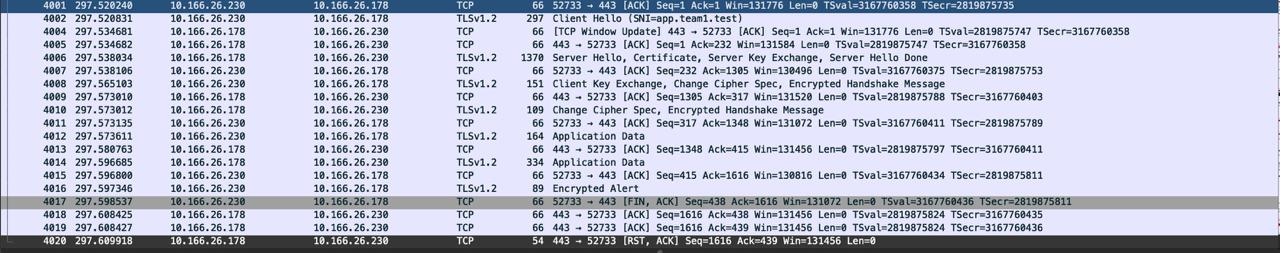
\includegraphics[width=\columnwidth]{G-tcp-handshake.png}\\[3pt]
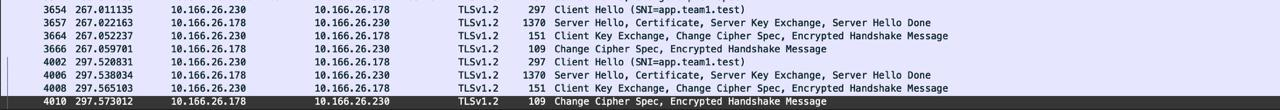
\includegraphics[width=\columnwidth]{G-tls-handshake.png}
\caption{Top: connection on port 52733 from the end of the handshake to teardown. Bottom: TLS~1.2 handshake records (ClientHello, ServerHello with Certificate, key exchange, ChangeCipherSpec).\src{G-wireshark/}}
\label{fig:tcp}
\end{figure}

\textit{Encryption and TLS termination.} After ChangeCipherSpec, Wireshark sees only TLS records of type Application Data whose payload is unreadable, because it does not hold the session keys negotiated in the handshake (Fig.~\ref{fig:enc}). Capturing Mac~2's loopback interface with \cmd{tcpdump} shows the other side of TLS termination: the request from nginx to the backend and the reply ``hello from backend A'' in plain text (Fig.~\ref{fig:plain}).

\begin{figure}[htbp]
\centerline{\includegraphics[width=\columnwidth]{G-encrypted-data.png}}
\caption{An Application Data record: the HTTP payload is encrypted.\src{G-wireshark/G-encrypted-data.png}}
\label{fig:enc}
\end{figure}

\begin{figure}[htbp]
\centerline{\includegraphics[width=\columnwidth]{G-internal-plaintext.png}}
\caption{Plain HTTP between nginx and a backend on Mac~2's loopback interface.\src{G-wireshark/G-internal-plaintext.png}}
\label{fig:plain}
\end{figure}

Table~\ref{tab:layers} maps the protocols of this request to the OSI and TCP/IP models.

\begin{table}[htbp]
\caption{Protocols of One Request by Layer}
\label{tab:layers}
\centering
\begin{tabular}{@{}l l l@{}}
\toprule
Protocol & OSI layer & TCP/IP layer \\
\midrule
DNS, HTTP & 7 Application & Application \\
TLS & 5--6 Session/Presentation & Application (over TCP) \\
TCP 443, UDP 53 & 4 Transport & Transport \\
IPv4 & 3 Network & Internet \\
Wi-Fi (802.11) & 2 Data link & Link \\
\bottomrule
\end{tabular}
\end{table}

\section{Failure Demonstrations}\label{sec:fail}
Each fault was injected, observed and reverted. Table~\ref{tab:fail} summarises them and Figs.~\ref{fig:f1}--\ref{fig:f5} show the evidence.

\begin{table*}[htbp]
\caption{Failure Demonstrations}
\label{tab:fail}
\centering
\begin{tabular}{@{}>{\raggedright}p{3.4cm} >{\raggedright}p{6.6cm} l >{\raggedright\arraybackslash}p{4.3cm}@{}}
\toprule
Fault & Observation & Layer & Lesson \\
\midrule
Client DNS set to 8.8.8.8 & \cmd{NXDOMAIN} from 8.8.8.8 with an SOA from the root servers; the network still works & DNS & DNS and IP connectivity are independent \\
Record points to a wrong IP & Name resolves to 10.166.26.250; the connection times out & DNS data & DNS is a directory, not a connection \\
Backend B stopped & Every response comes from Backend A; no request fails & Upstream & nginx retries on the healthy backend \\
Both backends stopped & DNS, TCP and TLS succeed; nginx returns \cmd{502 Bad Gateway} & Upstream & The 502 is generated by the edge \\
Port 8443 instead of 443 & \cmd{Connection refused} from 10.166.26.178 & Transport & Ports and addresses are separate identifiers \\
\bottomrule
\end{tabular}
\end{table*}

\begin{figure}[htbp]
\centerline{\includegraphics[width=\columnwidth]{fail-1-wrong-dns-server.png}}
\caption{Wrong DNS server: the public resolver returns NXDOMAIN for the private name.\src{failures/fail-1-wrong-dns-server.png}}
\label{fig:f1}
\end{figure}

\begin{figure}[htbp]
\centerline{\includegraphics[width=\columnwidth]{fail-2-wrong-record.png}}
\caption{Wrong record: the name resolves to a host that does not exist and the connection times out.\src{failures/fail-2-wrong-record.png}}
\label{fig:f2}
\end{figure}

\begin{figure}[htbp]
\centerline{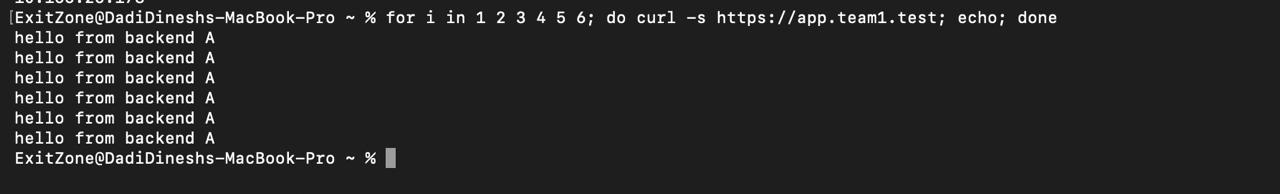
\includegraphics[width=\columnwidth]{fail-3-one-backend-down.png}}
\caption{One backend stopped: all requests are served by Backend A.\src{failures/fail-3-one-backend-down.png}}
\label{fig:f3}
\end{figure}

\begin{figure}[htbp]
\centerline{\includegraphics[width=0.62\columnwidth]{fail-4-both-backends-502.png}}
\caption{Both backends stopped: the TLS handshake succeeds and nginx returns 502 Bad Gateway.\src{failures/fail-4-both-backends-502.png}}
\label{fig:f4}
\end{figure}

\begin{figure}[htbp]
\centerline{\includegraphics[width=\columnwidth]{{fail-5-wrong-port.png}.jpeg}}
\caption{Wrong port: the host is reachable but nothing listens on 8443, so the connection is refused.\src{failures/fail-5-wrong-port.png.jpeg}}
\label{fig:f5}
\end{figure}

\section{Lessons Learned}\label{sec:lessons}
\textit{A host firewall can look like a network fault.} The first plan placed DNS on the laptop that became Mac~1. dnsmasq answered on 127.0.0.1 but timed out on the laptop's own LAN address, even when queried from the same machine. Layer by layer, \cmd{ping} worked, \cmd{lsof} showed dnsmasq bound to the LAN address, and \cmd{tcpdump} showed queries arriving with no replies; \cmd{profiles status} and \cmd{socketfilterfw} then showed a college-managed (MDM) laptop whose firewall policy cannot be changed by the user, along with a proxy network extension. Loopback traffic is not filtered, the LAN interface is. We therefore moved all server roles to Mac~2.

\textit{Configuration follows the network.} The hotspot assigned new addresses on reconnection, so the resolver's \cmd{listen-address} and records had to be updated each session. An IPv6 resolver advertised by the hotspot was also queried before ours and returned NXDOMAIN for \cmd{.test}.

\textit{Evidence beats assertion.} Each task was considered complete only when a tool showed the expected result from the client side: \cmd{dig}'s answer, \cmd{curl -v}'s ``verify ok'', a 304, or the packets themselves.

\section{Conclusion}
We built a private service network on two laptops in which a client resolves a private name through our own DNS server, connects over HTTPS to a reverse proxy that terminates TLS with a locally issued certificate, and is load-balanced across two backends, with HTTP caching on one endpoint. Packet captures show the DNS query on UDP 53, the TCP handshake on port 443, the TLS handshake and the encrypted application data, and five injected faults confirm which layer each component occupies. The main limitation is that Mac~2 is a single point of failure; Phase~2 addresses this with a backup resolver, firewall isolation, failover and a DNS-based edge migration.

\begin{thebibliography}{00}
\bibitem{rfc1034} P. Mockapetris, ``Domain names---concepts and facilities,'' RFC 1034, IETF, Nov. 1987.
\bibitem{rfc6761} S. Cheshire and M. Krochmal, ``Special-use domain names,'' RFC 6761, IETF, Feb. 2013.
\bibitem{rfc8446} E. Rescorla, ``The Transport Layer Security (TLS) protocol version 1.3,'' RFC 8446, IETF, Aug. 2018.
\bibitem{rfc9111} R. Fielding, M. Nottingham and J. Reschke, ``HTTP caching,'' RFC 9111, IETF, Jun. 2022.
\bibitem{nginxup} NGINX, ``Module ngx\_http\_upstream\_module,'' nginx documentation. [Online]. Available: \url{https://nginx.org/en/docs/http/ngx_http_upstream_module.html}
\bibitem{dnsmasq} S. Kelley, ``dnsmasq,'' manual page. [Online]. Available: \url{https://thekelleys.org.uk/dnsmasq/docs/dnsmasq-man.html}
\bibitem{express} OpenJS Foundation, ``Express---Node.js web application framework.'' [Online]. Available: \url{https://expressjs.com}
\end{thebibliography}

\end{document}
